% !TeX spellcheck = en_US

\chapter{Selective Quantification of \Acs{pe}, \Acs{pp}, and \Acs{ps} Plastic Debris in Soil by \Acs{py-gc-ms}}
\label{ch:py-gc-ms-method}

\paragraph{Abstract} The lack of adequate analytical methods\marginnote{This chapter was adapted from: \fullcite{SteinmetzSimple2020}.\par See Page~\pageref{ch:author-contributions} for \nameref{ch:author-contributions}.} for the quantification of plastic debris in soil challenges a better understanding of their occurrence and fate in the terrestrial environment.
With this proof-of-principle study, we developed a simple and fast method for the selective quantification of the three most environmentally relevant polymers \ac{pe}, \ac{pp}, and \ac{ps} in soil using \ac{py-gc-ms}.
In order to facilitate the preparation of calibration series and to better account for the heterogeneity of soil matrix, polymers were dissolved in \ac{tcb} at \SI{120}{\degreeCelsius}. Thereby, liquid sample aliquots from up to \SI{4}{\gram} of solid sample became amenable to pyrolysis without further preparation. To evaluate the performance of this approach, three reference soils with \SIrange{1.73}{5.16}{\percent} \ac{Corg} were spiked at \SIlist{50;250}{\micro\gram\per\gram} of each polymer and extracted with \ac{tcb}. Prior cleanup steps with methanol, flocculation with \ch{KAl(SO4)2}, or Fenton digestion were tested for their suitability to reduce potentially interfering \ac{Corg}.
Calibration curves responded linearly (adj. $R^2 > 0.996$) with instrumental \acp{lod} of \SIrange{1}{86}{\nano\gram} corresponding to estimated method \acp{lod} of \SIrange{1}{86}{\micro\gram\per\gram}. The measurement repeatability was \SIrange{3.2}{7.2}{\percent} \ac{rsd}. Recoveries of \SIrange{70}{128}{\percent} were achieved for plastic contents of \SI{250}{\micro\gram\per\gram} extracted with \ac{tcb} without prior cleanup from soils with less than \SI{2.5}{\percent} \ac{Corg}. A higher \ac{Corg} particularly interfered with the quantification of \ac{pe}. The addition of non-target polymers (\ac{pet}, \ac{pvc}, \ac{pmma}, and \ac{twp}) did not interfere with the quantification of the analytes highlighting the selectivity of the method. Further research is needed to determine low plastic contents in soils exceeding \SI{2.5}{\percent} \ac{Corg}. With \SIrange{1}{3}{\hour} processing time per sample, our method has the potential for routine analyses and screening studies of agricultural systems to be complemented with microspectroscopic techniques for additional information on particle shapes and sizes.

\section{Introduction}

The majority of plastic is produced, used, and disposed of on land, where it probably disintegrates into smaller debris such as microplastics (\SIrange{1}{1000}{\micro\meter}) or even nanoplastics (\SI{<1}{\micro\meter}) \citep{HartmannAre2019,HurleyFate2018,WagnerThings2019}. Whereas previous research has mainly focused on studying plastic debris in the aquatic environment, it remains unknown how and in which quantities such particles may distribute in terrestrial systems and particularly in soil. Currently, atmospheric deposition, littering, sewage sludge or biosolid applications, and use of agricultural plastic films are being discussed as potential sources of terrestrial plastic pollution, with \ac{pe}, \ac{pp}, \ac{ps}, and \ac{pet} as the most relevant polymers of interest \citep{HurleyFate2018,WangMicroplastics2019}.

Developing a better understanding of the occurrence and fate of plastic debris in the terrestrial environment requires reliable, quantitative analytical methods for complex environmental matrices \citep{BlasingPlastics2018,HeMicroplastics2018,daCostaMicroplastics2018}. So far, most studies have relied on optical detection by \ac{ftir} or Raman microspectroscopy \citep{RennerAnalytical2018}. Both techniques require extensive sample pretreatment to separate the plastic particles from sample matrix without losing the polymer analyte \citep{HurleyValidation2018}. When analyzing more complex matrices such as soil or organic wastes, sample preparation may easily take days or weeks \citep{LoderEnzymatic2017}. In addition, particle identification becomes prone to false positive detections, for example, by mistaking natural fibers or sand grains for plastic debris \citep{BlasingPlastics2018}. While this complicates a reliable quantification, microspectroscopic techniques provide valuable information about particle shapes and sizes. \citet{ScheurerMicroplastics2018} were the first who successfully developed and applied a method for the quantification of plastic debris in soil using a combination of density separation and oxidative matrix digestion followed by \ac{ftir} microspectroscopy. With their procedure, the authors obtained recoveries of \SIrange{93}{98}{\percent} and found a plastic content averaging \SI{5}{\micro\gram\per\gram} in Swiss floodplain soil. However, plastic contents were estimated from particle counts (\numrange{0}{600}\,particles\,\si{\per\kilo\gram}), sizes, and densities without stating \acp{lod} or \acp{loq}. Similarly, \citet{PiehlIdentification2018} screened agricultural soil for plastic debris and found \num{0.3(4)}\,particles\,\si{\per\kilo\gram}, but neglected debris smaller than \SI{1}{\milli\meter} due to the challenging sample pretreatment.

In such cases, thermoanalytical techniques such as \ac{tga-ms} \citep[Chapter~\ref{ch:tga-ms-method};][]{DavidIntroducing2019}, \ac{py-gc-ms} \citep{FischerSimultaneous2017,FischerMicroplastics2019}, or combinations of \ac{tga} with \acs{gc-ms} namely \ac{ted-gc-ms} \citep{DumichenAnalysis2015,DuemichenAutomated2019} may demonstrate their inherent benefits. All these methods are based on thermal decomposition of polymer mixtures at temperatures \SI{>500}{\degreeCelsius} and their quantification via characteristic indicator pyrolysates. Currently, instrumental \acp{lod} range from \SIrange[range-phrase = { to }]{3}{200}{\nano\gram} for \ac{ps} \citep{FischerMicroplastics2019,DuemichenAutomated2019} and up to \SIrange{0.5}{50}{\micro\gram} for \ac{pe}, \ac{pp}, and \ac{pet} \citep[Chapter~\ref{ch:tga-ms-method};][]{DuemichenAutomated2019}. In contrast to microspectroscopic methods, thermoanalytical techniques are assumed to be more robust against impurities from sample matrix. Yet, interferences may occur when pyrolysis products in plastic and matrix are identical. In addition, thermoanalytical measurements are typically restricted to sample amounts \SI{<100}{\milli\gram}, which puts high, hardly attainable requirements on sample homogeneity.

These challenges may be overcome by combining an adequate sample pretreatment with the selectivity of \ac{py-gc-ms} analyses. Therefore, we developed and validated a new \ac{py-gc-ms} method for the quantification of \ac{pe}, \ac{pp}, and \ac{ps} by using \ac{tcb} as a solvent both for the preparation of readily measurable polymer standards and for the extraction of plastic debris from different soil types. \Ac{tcb} is a typical eluent for \ac{sec} of polymers \citep{BivensPolymertoSolvent2016} and has been assessed for quantitative \ac{hnmr} of polymers \citep{PeezFirst2019}. Recently, \citet{DierkesQuantification2019} took a comparable approach by extracting \ac{pe}, \ac{pp}, and \ac{ps} with \ac{thf} from various solid matrices using \ac{ase}. Although the polymers needed to be reprecipitated in silica gel and could not be analyzed directly via \ac{py-gc-ms}. Unlike \ac{thf}, \ac{tcb} is not classified as teratogenic and has a more than 100-fold lower vapor pressure according to the respective material and safety data sheets. This makes \ac{tcb} easy to handle in batch extraction set-ups. Moreover, sample pretreatment and extraction can be carried out in a single tube which reduces the contamination potential and facilitates scalability for routine analyses.

\section{Material and Methods}

\subsection{Preparation of Polymer Standards}

The polymers used in this study were \ac{pe} beads of \SI{500}{\micro\meter} average particle size \sidenote{\cas{9002-88-4}, Alfa Aesar, Kandel, Germany.}, isotactic \ac{pp} pellets\sidenote{\cas{9003-07-0}, Aldrich Chemistry, Taufkirchen, Germany.}, and \ac{ps} particles with an average particle size of \SI{250}{\micro\meter}\sidenote{\cas{9003-53-6}, Goodfellow, Huntingdon, UK.}. The \ac{pp} pellets were ground using a commercially available coffee mill with stainless steal lining\sidenote{Cloer 7580, Arnsberg, Germany.} to pass a \SI{1000}{\micro\meter} sieve. All polymer standards were prepared in \ac{tcb}\sidenote{\cas{120-82-1}, \SI{99}{\percent} purity, Alfa Aesar, Kandel, Germany.} containing \SI{0.015}{\percent} \ac{bht}\sidenote{\cas{128-37-0}, \SI{>=99}{\percent} purity, Merck, Darmstadt, Germany.} as antioxidant \citep{BivensPolymertoSolvent2016}. To this end, \SI{50}{\milli\gram} of \ac{pe}, \ac{pp}, and \ac{ps} were weighed individually and as an equal mixture of all three polymers into glass culture tubes\sidenote{16 \texttimes\ \SI{100}{\square\milli\meter}, GL18, VWR, Darmstadt Germany.}. The tubes were equipped with \iac{pbt} screw cap and \iac{ptfe}-coated sealing\sidenote{Carl Roth, Karlsruhe, Germany.}. The plastic particles were mixed with \SI{5}{\milli\liter} of \ac{tcb} and heated to \SI{120}{\degreeCelsius} for \SI{30}{\minute} to facilitate dissolution. After having cooled down to room temperature, the polymers formed a sol-like phase within the \ac{tcb} that could easily be dispersed upon manual agitation before diluting the polymer standards. Dilution series of \SIlist{5;10;20;50;100;150}{\micro\gram\per\milli\liter} were prepared using \SIrange{10}{100}{\micro\liter} positive displacement pipettes with glass capillaries\sidenote{Transferpettor micro, Brand, Wertheim, Germany.} and \SIrange{2}{5}{\milli\liter} volumetric glass flasks. Standard solutions were kept in \SI{2}{\milli\liter} ND9 glass vials with \ac{ptfe}\-/sealed caps.

\subsection{Extraction of Plastic Debris from Soil}

For the recovery experiment, three soils with different textures and \ac{Corg} contents were selected (Table~\ref{tab:soil-properties}). RefeSol 06-A\sidenote{Fraunhofer IME, Schmallenberg, Germany.} and LUFA~2.2\sidenote{\foreignlanguage{ngerman}{Landwirtschaftliche Untersuchungs- und Forschungsanstalt}, Speyer, Germany.} as used in Chapter~\ref{ch:tga-ms-method} served as reference soils from organically managed arable areas. In addition, a pristine forest soil was taken from a continuous observation site in Wallmerod (WR)\sidenote{\foreignlanguage{ngerman}{Landesamt für Geologie und Bergbau}, Rhineland-Palatinate, Germany.} \citep{MeyerDetermination2018}. None of the suppliers provided information on polymer background levels.

\begin{table}[b]
	\centering\footnotesize
	\caption{Overview of physicochemical soil properties.}\label{tab:soil-properties}
	\begin{tabular}{llSSSSS}
		\toprule
		{Soil} & {Texture} & {Clay} & {Silt} & {Sand} & {pH} & {C\textsubscript{org}} \\
		& & [\si{\percent}] & [\si{\percent}] & [\si{\percent}] & & [\si{\percent}] \\
		\midrule
		RefeSol 06-A & Silty clay & 47.2 & 41.3 & 11.5 & 7.39 & 2.5 \\
LUFA 2.2 & Loamy sand & 8.6 & 15.7 & 75.7 & 5.6 & 1.73 \\
WR & Clayey silt & 25.0 & 70.0 & 5.0 & 5.0 & 5.16 \\
		\bottomrule
	\end{tabular}
\end{table}

In order to assess the efficacy of \ac{tcb} for extracting \ac{pe}, \ac{pp}, and \ac{ps} from different soil types, soil triplicates of \SI{4}{\gram} were weighed into glass culture tubes and spiked with \SIlist{0.2; 1.0}{\milli\gram} \ac{pe}, \ac{pp}, and \ac{ps} using a microscale\sidenote{Sartorius SE 02-OCE, Göttingen, Germany.}. With that, a nominal content of \SIlist{50;250}{\micro\gram\per\gram} of each polymer was obtained. Soil without any plastic supplement served as control. One batch of LUFA~2.2 soil was further spiked with \SI{0.2}{\milli\gram} of plastics not targeted in our analysis to evaluate whether their pyrolysates interfere with \ac{pe}, \ac{pp}, and \ac{ps} extraction and quantification. This non-target plastic mixture consisted of \SI{19}{\percent} \ac{pet} from recycled bottles\sidenote{PETKA CZ, Brno, Czech Republic.}, \SI{11}{\percent} \ac{pmma} ground from a commercial plexiglass\sidenote{\foreignlanguage{ngerman}{Bundesanstalt für Materialforschung und -prüfung}, Berlin, Germany.}, \SI{41}{\percent} \ac{pvc}\sidenote{Aldrich Chemistry, Taufkirchen, Germany.}, and \SI{29}{\percent} \ac{twp} from a test rig\sidenote{\foreignlanguage{ngerman}{Bundesanstalt für Straßenwesen, Bergisch Gladbach}, Germany.}. Content and composition of the non-target polymers were based on findings by \citet{PiehlIdentification2018} to reflect realistic conditions in agricultural soil.

Since natural soil polymers may also interfere with plastic quantification, additional sample cleanup procedures were tested for WR soil with \iac{Corg} of \SI{5.16}{\percent}. The selected cleanup procedures were intended to be fast (\SI{<2}{\hour} processing time for a 12-sample batch), easily scalable and reproducible, robust against external contamination, and compatible with the subsequent dissolution of polymers in \ac{tcb}.
To this end, soil \ac{Corg} was either preextracted with methanol, oxidatively digested using Fenton reagent, or flocculated with \ch{KAl(SO4)2} prior to \ac{tcb} extraction.
The methanol cleanup was simplified from \citet{FullerProcedure2016}. In brief, spiked soils were topped off with \SI{8}{\milli\liter} methanol\sidenote{\cas{67-56-1}, \SI{99.9}{\percent}, Carl Roth, Karlsruhe, Germany.} and agitated for \SI{60}{\minute} in a horizontal shaker at \SI{150}{rpm}. Afterwards, the extracts were centrifuged at \SI{1500}{rcf} for \SI{15}{\minute} and the supernatant was discarded. The remaining methanol was evaporated at \SI{60}{\degreeCelsius} under a gentle \ch{N2} stream.
The Fenton digestion was performed by adding \SI{10}{\milli\liter} of aqueous \ch{FeSO4 * 7 H2O} solution\sidenote{\cas{7782-63-0}, \SI{20}{\gram\per\liter}, pH~2, Carl Roth, Karlsruhe, Germany.} and \SI{10}{\milli\liter} of \ch{H2O2}\sidenote{\cas{7722-84-1}, \SI{30}{\percent}, Carl Roth, Karlsruhe, Germany.} to the spiked soil in accordance with \citet{HurleyValidation2018}. The reaction mixture was left for \SI{60}{\minute} in an ice bath before slowly heating it to \SI{60}{\degreeCelsius} to dry the sample and decompose remaining \ch{H2O2}.
Humic substances were flocculated by mixing \SI{4}{\milli\liter} of a \SI{500}{\milli\gram\per\liter} aqueous \ch{KAl(SO4)2 * 12 H2O} solution\sidenote{\cas{7784-24-9}, \SI{>=98}{\percent}, Carl Roth, Karlsruhe, Germany.} with the soil \citep{MandalakisSimple2018}. The mixture was shaken for \SI{60}{\minute} at \SI{150}{rpm} and evaporated under \ch{N2} at \SI{105}{\degreeCelsius}.

Finally, all soil samples were extracted with \SI{8}{\milli\liter} \ac{tcb} at \SI{120}{\degreeCelsius} for \SI{60}{\minute}. After having cooled down, the extracts were allowed to sediment before transferring the supernatant into ND9 vials using glass Pasteur pipettes. Procedural blanks and control soil without any plastic added followed all extraction steps to quantify a potential contamination.

\subsection{\Acs{py-gc-ms} Analysis}

Instrumental analyses were performed using a Pyroprobe 6150 filament pyrolyzer\sidenote{CDS Analytical, Oxford, US.} coupled with a Trace GC Ultra with DSQII \ac{ms}\sidenote{Thermo Fisher Scientific, Bremen, Germany.}. The pyrolyzer probe consists of a resistively heated platinum coil that holds an open ended quartz tube. The quartz tubes were filled with two quartz filter disks punched out of a high\-/purity microfiber filter\sidenote{Whatman QM-A, Kent, UK.} using a \SI{2}{\milli\meter} biopsy punch with plunger\sidenote{Miltex, Rietheim-Weilheim, Germany.}. The filter disks were positioned inside the quartz tube so that they align with the center of the platinum coil when placed into the pyrolyzer probe (Figure~\ref{fig:quartz-tube}).

\begin{marginfigure}
	\centering
	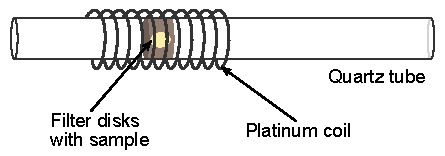
\includegraphics[width=\marginparwidth]{figures/quartz-tube}
	\caption{Schematic of a pyrolyzer quartz tube equipped with filter disks to absorb the liquid sample.}
	\label{fig:quartz-tube}
\end{marginfigure}

Prior to \ac{py-gc-ms} analysis, a sample aliquot of \SI{2}{\micro\liter} was applied onto the filter disk inside the quartz tube using a gastight \SI{10}{\micro\liter} syringe with \ac{ptfe} plunger\sidenote{Hamilton 1701 N with 26s gauge, Bonaduz, Switzerland.}. The quartz tube was transferred into the pyrolyzer using stainless steal tweezers to avoid any contamination, for instance, from nitrile or latex gloves. The pyrolyzer interface was held at \SI{300}{\degreeCelsius} and continuously flushed with \SI{20}{\milli\liter\per\minute} \ch{He} to evaporate remaining \ac{tcb} (boiling point: \SI{213}{\degreeCelsius}) and volatiles on-line while remaining below \ac{pe}, \ac{pp}, and \ac{ps} degradation onsets of \SIrange{310}{350}{\degreeCelsius} \citep{DavidIntroducing2019}. After \SI{3}{\minute}, the sample was flash pyrolyzed (\SI{10}{\kelvin\per\milli\second}) at \SI{750}{\degreeCelsius} for \SI{15}{\second}. The pyrolysis temperature was chosen following the manufacturer's recommendation to overcome the heat resistance of the pyrolyzer quartz tube ensuring complete thermal degradation of the polymers. The pyrolysates were transferred to the \ac{gc-ms} system via a passivated transfer line (\SI{350}{\degreeCelsius}). The \ac{ssl} injector was operated at \SI{300}{\degreeCelsius} with a split ratio of 1:10. The pyrolysates were separated on a \SI{30}{\meter} \texttimes\ \SI{0.25}{\milli\meter} capillary column (\SI{5}{\percent} phenyl-arylene, \SI{95}{\percent} dimethylpolysiloxane, \SI{0.25}{\micro\meter} film thickness)\sidenote{ZB-5MS, Phenomenex, Aschaffenburg, Germany.} connected to a \SI{2}{\meter} deactivated fused silica guard column\sidenote{Phenomenex, Aschaffenburg, Germany.}. The \ch{He} carrier gas flow was set at \SI{1.3}{\milli\liter\per\minute}. The \ac{gc} oven was programmed from \SI{40}{\degreeCelsius} (\SI{2}{\minute} hold) to \SI{300}{\degreeCelsius} at \SI{8}{\kelvin\per\minute} (\SI{50}{\minute} run time). The transfer line connecting the \ac{gc} with the \ac{ms} was kept at \SI{280}{\degreeCelsius}, and the \ac{ms} ion source (\ac{ei}, \SI{70}{\electronvolt}) was heated to \SI{230}{\degreeCelsius}.
The fore pressure of the \ac{ms} was checked to be \SI{<0.07}{\milli\bar}. The background intensity of \SI{28}{\mz} (atmospheric \ch{N2}) was supposed to be \num{<5e7} and the \ac{tic} \num{<e8}. Values exceeding these criteria indicated a leak in the system.

\subsection{Pyrolysate Identification and Calibration}

Pyrolysates were first screened in scan mode (\SIrange{50}{300}{\mz}) before switching to \ac{sim} of specific \si{\mz} ratios (\SI{100}{\milli\second} dwell time) as indicated in Figure~\ref{fig:py-sample} and Table~\ref{tab:py-products} and reported in previous research \citep{TsugePyrolysis2011,FischerSimultaneous2017,DumichenAnalysis2015}. \Ac{tic} pyrograms were evaluated using OpenChrom (Community Edition version 1.4.0)\sidenote{Lablicate, Hamburg, Germany.} \citep{WenigPostoptimization2011} with NIST08 database for peak identification. Identified pyrolysates (Table~\ref{tab:py-products}) were abbreviated based on a modified ``lipid number'' notation in the form of $b$$C$:$D$($p_1$, $p_2$, \dots, $p_{D/2}$), in which $C$ is the total number of carbon atoms of the compound, $D$ denotes the number of double bonds, and their respective position $p$ is given in parentheses \citep{ZellesFatty1999}. The prefix $b$ specifies additional functional groups and their position in the carbon backbone, for example, 2Me for a methyl group or 2Ph for a phenyl moiety at the second carbon atom.

\begin{figure*}
	\centering
	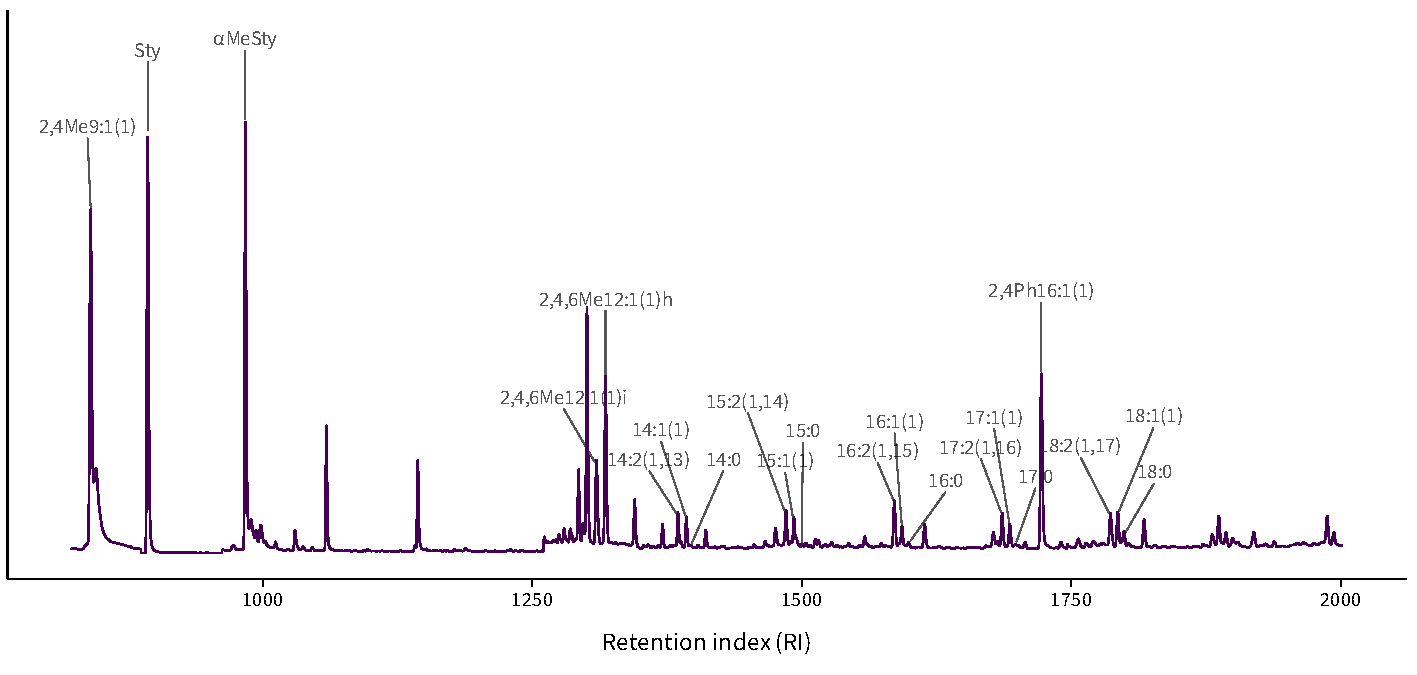
\includegraphics[width=\textwidth]{figures/py-sample}
	\caption[Sample pyrogram of \iac{pe}, \ac{pp}, and \ac{ps} mixture.]{Sample pyrogram of a polymer mixture containing each  \SI{150}{\micro\gram\per\gram} \ac{pe}, \ac{pp}, and \ac{ps}; see Table~\protect\ref{tab:py-products} for details.}
	\label{fig:py-sample}
\end{figure*}

\begin{table*}
	\centering\footnotesize
	\caption{\Ac{pe}, \ac{pp}, and \ac{ps} pyrolysates analyzed for \ac{py-gc-ms} method development.}\label{tab:py-products}
	\begin{tabular}{llllS[table-format = 4]l}
		\toprule
		{Polymer} & {Pyrolysate} & {Full name} & {CAS} & {\acs{ri}} & {\si{\mz}} \\
		\midrule
		PE & 14:2(1,13) & 1,13-Tetradecadiene & \cas[]{021964-49-8} & 1385 & \numlist[list-pair-separator = {, }]{82;95} \\
 & 14:1(1) & 1-Tetradecene & \cas[]{001120-36-1} & 1392 & \numlist[list-final-separator = {, }]{55;69;83}\textsuperscript{\textdaggerdbl} \\
 & 14:0 & Tetradecane & \cas[]{000629-59-4} & 1400 & \numlist[list-final-separator = {, }]{55;69;83}\textsuperscript{\textdaggerdbl} \\
 & 15:2(1,14) & 1,14-Pentadecadiene & \cas[]{021964-50-1} & 1485 & \numlist[list-pair-separator = {, }]{82;95} \\
 & 15:1(1) & 1-Pentadecene & \cas[]{013360-61-7} & 1493 & \numlist[list-final-separator = {, }]{55;69;83}\textsuperscript{\textdaggerdbl} \\
 & 15:0 & Pentadecane & \cas[]{000629-62-9} & 1500 & \numlist[list-final-separator = {, }]{55;69;83}\textsuperscript{\textdaggerdbl} \\
 & 16:2(1,15) & 1,15-Hexadecadiene & \cas[]{021964-51-2} & 1585 & \numlist[list-pair-separator = {, }]{82;95} \\
 & 16:1(1) & 1-Hexadecene & \cas[]{113032-42-1} & 1593 & \numlist[list-final-separator = {, }]{55;69;83}\textsuperscript{\textdaggerdbl} \\
 & 16:0 & Hexadecane & \cas[]{000544-76-3} & 1600 & \numlist[list-final-separator = {, }]{55;69;83}\textsuperscript{\textdaggerdbl} \\
 & 17:2(1,16) & 1,16-Heptadecadiene & \cas[]{021964-52-3} & 1686 & \numlist[list-pair-separator = {, }]{82;95} \\
 & 17:1(1) & 1-Heptadecene & \cas[]{006765-39-5} & 1693 & \numlist[list-final-separator = {, }]{55;69;83}\textsuperscript{\textdaggerdbl} \\
 & 17:0 & Heptadecane & \cas[]{000629-78-7} & 1700 & \numlist[list-final-separator = {, }]{55;69;83}\textsuperscript{\textdaggerdbl} \\
 & 18:2(1,17) & 1,17-Octadecadiene & \cas[]{013560-93-5} & 1787 & \numlist[list-pair-separator = {, }]{82;95} \\
 & 18:1(1) & 1-Octadecene & \cas[]{000112-88-9} & 1793 & \numlist[list-final-separator = {, }]{55;69;83}\textsuperscript{\textdaggerdbl} \\
 & 18:0 & Octadecane & \cas[]{000593-45-3} & 1800 & \numlist[list-final-separator = {, }]{55;69;83}\textsuperscript{\textdaggerdbl} \\
PP & 2,4Me9:1(1) & 2,4-Dimethyl-1-heptene & \cas[]{19549-87-2} & 841 & \numlist[list-pair-separator = {, }]{70;126} \\
 & 2,4,6Me12:1(1)i & 2,4,6-Trimethyl-1-nonene (isotactic) & \cas[]{55771-40-9} & 1307 & \numlist[list-pair-separator = {, }]{69;111} \\
 & 2,4,6Me12:1(1)h & 2,4,6-Trimethyl-1-nonene (heterotactic) & \cas[]{55771-40-9} & 1316 & \numlist[list-pair-separator = {, }]{69;111} \\
PS & Sty & Styrene & \cas[]{100-42-5} & 895 & \numlist[list-pair-separator = {, }]{78;104} \\
 & $\alpha$MeSty & $\alpha$-Methylstyrene & \cas[]{98-83-9} & 981 & \numlist[list-pair-separator = {, }]{103;118} \\
 & 2,4Ph16:1(1) & 2,4-Diphenyl-1-butene & \cas[]{16606-47-6} & 1721 & \numlist[list-pair-separator = {, }]{91;208} \\
 & 2,4,6Ph24:1(1) & 2,4,6-Triphenyl-1-hexene & \cas[]{18964-53-9} & 2438 & \numlist[list-pair-separator = {, }]{91;207} \\
		\bottomrule
		\multicolumn{6}{l}{\acs{ri} = \acl{ri}; \textsuperscript{\textdaggerdbl}used for screening only.} \\
	\end{tabular}
\end{table*}

Peaks were automatically integrated from the valley between the peaks to the horizontal baseline using a sliding window size of 3~scans and a minimum \ac{snr} of~7.
Calibration series of \SIrange{5}{150}{\micro\gram\per\milli\liter} mixed \ac{pe}, \ac{pp}, and \ac{ps} standards were pyrolyzed together with \numrange{3}{5} blanks (\SI{0}{\micro\gram\per\milli\liter} in \ac{tcb}).
\Acp{lod} and \acp{loq} were calculated using Equations~\ref{eq:lod} and \ref{eq:loq} as described in Section~\ref{sec:tga-ms-analysis}.
%\Acp{lod} and \acp{loq} were calculated using Equations~\ref{eq:lod} and \ref{eq:loq}, respectively, in accordance with the German standard \citet{DIN32645Chemical2008} as implemented in the R package ``envalysis''\marginnote{The package source is available at \doi{10.5281/zenodo.1240305}} (version 0.3.3).
%
%\begin{equation}
%\mathrm{LOD} = \frac{\sigma_\mathrm{blank}}{a} \cdot t_{n-1;0.01} \sqrt{n^{-1} + m^{-1}}
%\label{eq:lod}
%\end{equation}
%
%\begin{equation}
%\mathrm{LOQ} = k \cdot \frac{\sigma_{xy}}{a} \cdot t_{n-2;0.01} \sqrt{n^{-1} + m^{-1} + \frac{(\mathrm{LOQ}-\overline{x})^2} {S_{xx}}}
%\label{eq:loq}
%\end{equation}
%
%Therein, $\sigma_\mathrm{blank}$ is the standard deviation of integrated peak areas from blanks, $\sigma_{xy}$ is the residual standard deviation, and $a$ is the slope of the calibration curve. $t$ is the \SI{99}{\percent} percentile of the Student's $t$ distribution with $n - 1$ and $n - 2$ degrees of freedom, $n$ as the total number of measurements, and $m$ as the number of replicates. $k = 3$ is the recommended certainty factor for the \ac{loq}; $\overline{x}$ is the arithmetic mean of all standard concentrations, and $S_{xx}$ is the sum of squares of $x$. Note that calculating the \ac{loq} is an iterative process with $\mathrm{LOQ} = k \cdot \mathrm{LOD}$ as initial value.
Instrumental \acp{lod} were calculated by multiplication of the respective \acp{lod} with the injection volume of \SI{2}{\micro\liter}. Method \acp{lod} were estimated by dividing \acp{lod} by the extraction volume of \SI{8}{\milli\liter} and multiplying it with the extracted soil mass (\SI{4}{\gram}).

\subsection{Method Validation}

At the beginning of each week, a fresh calibration series was prepared. Sample measurements of the following days were bracketed with \SI{100}{\micro\gram\per\milli\liter} standards to correct for inter-day variations in peak intensities. Corrected peak areas were then used for quantification.

In line with IUPAC recommendations \citep{CurrieNomenclature1995}, the intra-day repeatability of the \ac{py-gc-ms} method was verified by measuring a sequence of \SI{150}{\micro\gram\per\milli\liter} standards ($n = 10$) and determining \acp{rsd} of peak areas. A linear model was fitted to the data to check if the peak areas changed significantly during the day. Inter-day variability was estimated from two \SI{150}{\micro\gram\per\milli\liter} standard samples repeatedly measured for eight days.

In order to test whether \ac{pe}, \ac{pp}, and \ac{ps} selectively decompose into their respective pyrolysates without interfering with each other, successive measurements of \SI{150}{\micro\gram\per\milli\liter} mixed polymer standards were compared with standards containing each individual polymer. Furthermore, potential interferences from soil matrix and non-target plastics (\ac{pet}, \ac{pmma}, \ac{pvc}, and \ac{twp}) were assessed. Differences in peak areas of pyrolysates were statistically evaluated using \acp{anova} with Bonferroni\-/adjusted Tukey tests for post\-/hoc multiple comparisons. \Acp{anova} were checked for normality and homoscedasticity of residuals using quantile\--quantile and residual vs. fitted plots.
The same statistical tools were applied to compare the various extraction and cleanup methods for \ac{pe}, \ac{pp}, and \ac{ps} from different soil types with one another.
Data analysis was performed using R statistical software (version 3.6.1)\marginnote{All data and R code to reproduce data processing and statistical tests are publicly available at \doi{10.6084/m9.figshare.11861664}.}.
Results are given as mean$\pm$\ac{sd}.

\section{Results and Discussion}

\subsection{Polymer Quantification}

From the initial screening set of 22~pyrolysates (Table~\ref{tab:py-products}), six compounds performed best in terms of linearity (adj. $R^2$ \num{>0.996}) within the calibration range, \acp{lod}, and \acp{loq} (Figure~\ref{fig:py-calibration} and Table~\ref{tab:py-calibration}). \Acp{lod} were below the lowest standard of \SI{5}{\micro\gram\per\milli\liter} for the \ac{pe} $n$-alkadienes 15:2(1,14) and 17:2(1,16) detected via \SIlist{82;95}{\mz}. 18:2(1,17) produced \iac{lod} of \SI{11.3}{\micro\gram\per\milli\liter}. The \acp{loq} ranged between \SIrange[range-phrase = { and }]{25}{54}{\micro\gram\per\milli\liter}.
For \ac{pp}, only 2,4Me9:1(1) was quantifiable (\SIlist{70;126}{\mz}) with \iac{lod} and \ac{loq} of \SIlist{43.2;46.7}{\micro\gram\per\milli\liter}, respectively.
Sty and $\alpha$MeSty were the most indicative pyrolysates for \ac{ps} and detected via \SIlist{78;104}{\mz} and \SIlist{103;118}{\mz}, respectively. Their adj. $R^2$s, \acp{lod}, and \acp{loq} were similar to \ac{pe} pyrolysates.

\begin{figure*}
	\centering
	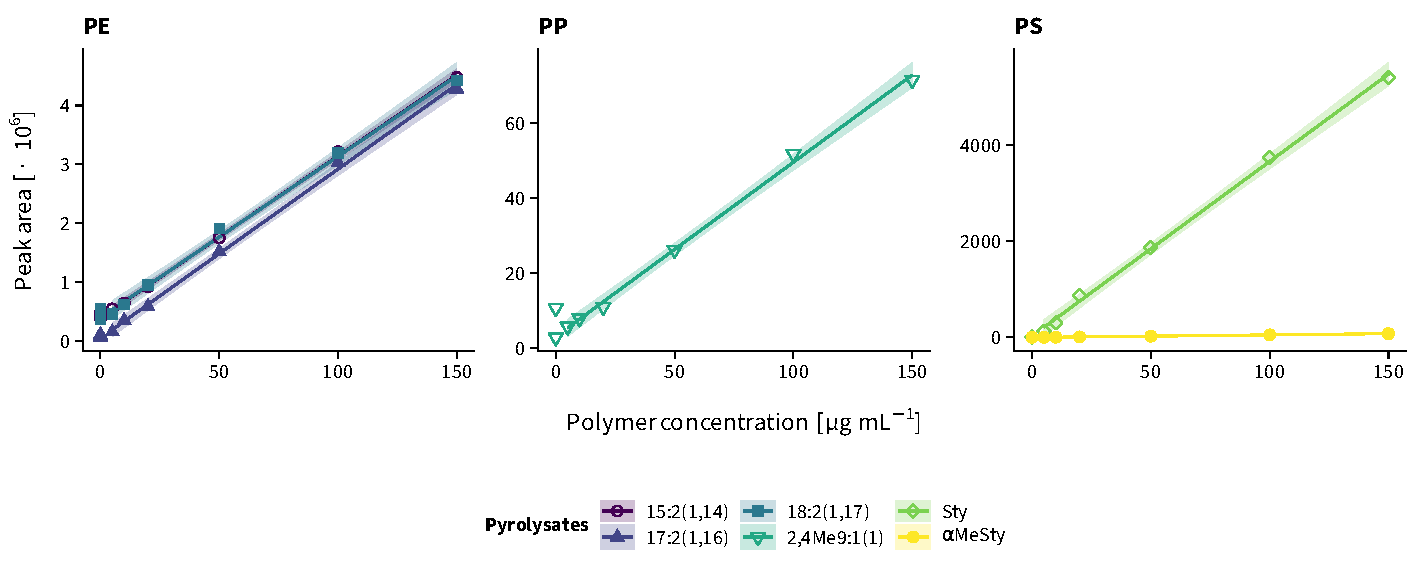
\includegraphics[width=\textwidth]{figures/py-calibration}
	\caption[\Ac{py-gc-ms} calibration curves of \ac{pe}, \ac{pp}, and \ac{ps} standards in \acs{tcb}.]{\Ac{py-gc-ms} calibration curves of \ac{pe}, \ac{pp}, and \ac{ps} standards in \acf{tcb}; see Table~\protect\ref{tab:py-calibration} for parameters.}
	\label{fig:py-calibration}
\end{figure*}

\begin{table}[b]
	\centering\footnotesize
	\caption{\Ac{py-gc-ms} calibration parameters of pyrolysates selected for quantification.}\label{tab:py-calibration}
	\begin{tabular}{llS[table-format = 8]S[table-format = 8]S[table-format = 1.4]S[table-format = 2.1]S[table-format = 2.1]}
		\toprule
		{Polymer} & {Pyrolysate} & {Intercept} & {Slope} & {adj. $R^2$} & {LOD} & {LOQ} \\
		& & & & & [\si{\micro\gram\per\milli\liter}] & [\si{\micro\gram\per\milli\liter}] \\
		\midrule
		PE & 15:2(1,14) & 384440 & 27563 & 0.9992 & 4.8 & 25.7 \\
 & 17:2(1,16) & 40501 & 28782 & 0.9980 & 2.5 & 38.6 \\
 & 18:2(1,17) & 391786 & 27423 & 0.9962 & 11.3 & 53.4 \\
PP & 2,4Me9:1(1) & 2987986 & 464559 & 0.9971 & 43.2 & 46.7 \\
PS & Sty & 26306594 & 36246576 & 0.9975 & 0.5 & 43.3 \\
 & $\alpha$MeSty & -860185 & 527700 & 0.9986 & 1.6 & 33.1 \\

		\bottomrule
	\end{tabular}
\end{table}

Taking into account the \SI{2}{\micro\liter} injection volume, instrumental \acp{lod} were \SIrange{1}{86}{\nano\gram}. This is at least \num{2.5} times lower than most recent advances in \ac{pe}, \ac{pp}, and \ac{ps} method developments with \ac{ted-gc-ms} and microfurnace \ac{py-gc-ms} \citep{DuemichenAutomated2019,FischerMicroplastics2019,DierkesQuantification2019}. Note that \citet{DierkesQuantification2019} reported \acp{loq} calculated from blanks, which is usually defined as \ac{lod} (Equation~\ref{eq:lod}). While \citet{DuemichenAutomated2019,DierkesQuantification2019} used the same indicator pyrolysates for quantification as we did but on different \si{\mz} ratios, \citet{FischerMicroplastics2019} chose $n$-alkanes, $n$-alkenes, and the \ac{ps} trimer 2,4,6Ph24:1(1).

All these studies have in common that they relied on a very sensitive microscale to weigh several nanograms of solid polymer directly into pyrolyzer sample cups or to quantitatively transfer a representative aliquot of solid mixture. To facilitate the heat transfer of the pyrolyzer filament or microfurnace into the sample, the lowest sample amount possible is typically aimed for. However, the lower the amount to be weighed, the higher the relative weighing error becomes and the more challenging it is to obtain a homogeneous mixture. So far, this has been one of the major drawbacks of \ac{py-gc-ms} \citep{FischerMicroplastics2019}.
When combining \ac{py-gc-ms} with prior dissolution of polymers in an appropriate solvent such as \ac{tcb}, stock solutions can be easily handled, quantitatively diluted or preconcentrated, and transferred directly into the pyrolyzer quartz tubes. Dissolution in \ac{tcb} therefore allows for constantly pyrolyzing the same but low amount of sample. Absorbing the \ac{tcb} solution into the quartz filter disks inside the quartz tube further ensures the optimal alignment of the sample with the pyrolyzer filament and thereby enabling more accurate and reproducible pyrolyses down to the nanogram range. Trying to further improve \acp{lod} and \acp{loq} by increasing sample injection volumes could therefore be at the expense of measurement accuracy.

\subsection{Repeatability}

The \acp{rsd} of \ac{pe} indicator pyrolysates were \SIrange{3.4}{4.5}{\percent} without showing any trend of systematically increasing or decreasing peak intensities during a one-day series of $n = 10$ standard measurements (Figure~\ref{fig:py-repeatability}, $p > 0.529$, linear model); this is intra-day variability. By contrast, inter-day variability was \SIrange{15.2}{17.9}{\percent}. The \ac{pp} pyrolysate 2,4Me9:1(1) produced a stable ($p = 0.728$, linear model) intra-day \ac{rsd} of \SI{7.2}{\percent}, and an inter-day \ac{rsd} of \SI{10.4}{\percent}. With \SIlist{3.2;4.2}{\percent} of intra-day variability, the \acp{rsd} of \ac{ps} pyrolysates Sty and $\alpha$MeSty were in the same range as \ac{pe}.  However, Sty showed a statistically significant tendency to decrease in signal intensity by \SI{0.88}{\percent} per measurement ($p = 0.002$, linear model), while $\alpha$MeSty increased by \SI{1.05}{\percent} ($p = 0.020$, linear model). With respect to the \acp{rsd} of the measurement series, these changes are deemed negligible if peak intensities are corrected with bracketing standards measured in the beginning and at the end of each day. This also applies to the inter-day variabilities of Sty and $\alpha$MeSty which were  \SIlist{13.9;16.5}{\percent}.

\begin{figure*}[t]
	\centering
	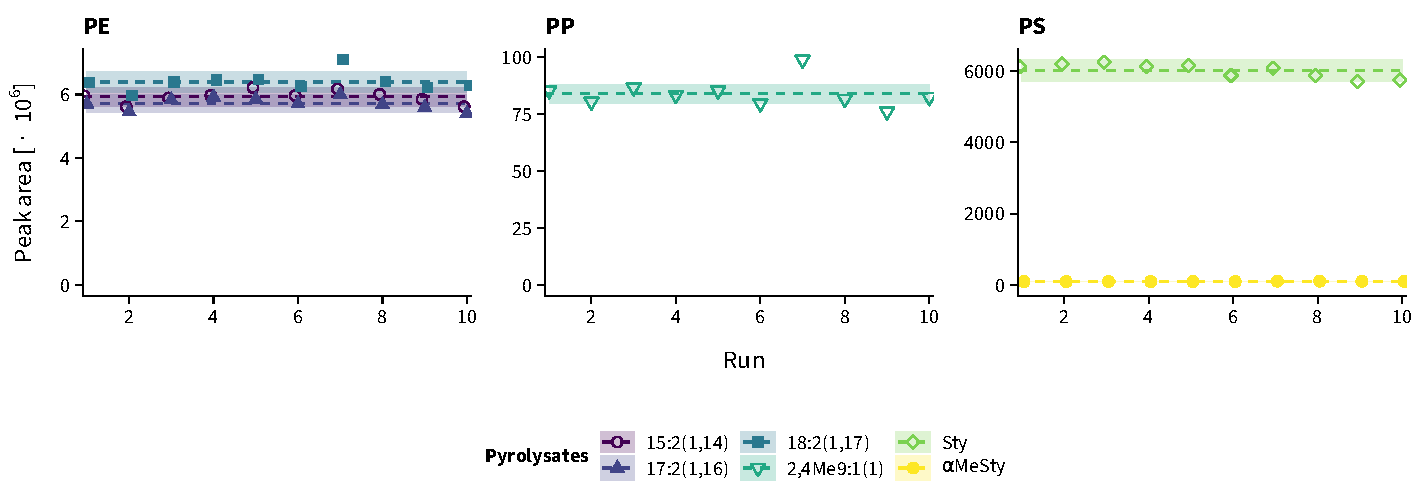
\includegraphics[width=\textwidth]{figures/py-repeatability}
	\caption[Repeatability of \ac{py-gc-ms} measurements.]{Repeatability of \ac{py-gc-ms} measurements ($n = 10$) with means (dashed lines) and \SI{+-5}{\percent} \acs{rsd} bands.}
	\label{fig:py-repeatability}
\end{figure*}

Measurement repeatability was in line with comparable studies. \Ac{ps} analysis via \ac{lc-ms} with an atmospheric pressure photoionization source, for instance, resulted in an intra- and inter-day repeatability of \SIrange{1.8}{2.4}{\percent} and \SIrange{15.5}{25.6}{\percent}, respectively ($n = 5$) \citep{SchirinziTrace2019}. With \ac{ted-gc-ms}, \citet{DuemichenAutomated2019} achieved \acp{rsd} ranging from \SIrange[range-phrase = { to }]{6}{12}{\percent} for various \ac{pp} pyrolysates. The authors suggested using an internal standard to further optimize \acp{rsd}. \citet{FischerMicroplastics2019} used androstane, deuterated anthracene, 9-dodecyl-1,2,3,4,5,6,7,8-octahydro anthracene, and cholanic acid for internal standardization of \ac{pe}, \ac{pet}, polycaprolactam, and \ac{ps}. Since those internal standards are not polymers, they probably behave differently than the polymer analytes when heated to typical pyrolysis temperatures of \SIrange{600}{800}{\degreeCelsius}. Particularly polycyclic aromatic hydrocarbons such as anthracene are thermally stable and more likely to evaporate instead of thermally decomposing along with the polymer analytes. Accordingly, \citet{FischerMicroplastics2019} reported that the deuterated anthracene might have interacted with the inner surface of the pyrolyzer which eventually decreased repeatability. Though expensive, deuterated plastics \citep{DierkesQuantification2019} or specialized polymers like \ac{pedot} typically used in semiconductor industry could be promising alternatives since they decompose in the same temperature range as the polymer analytes \citep{JinThermal2013}. The use of an appropriate internal standards for routine \ac{py-gc-ms} analyses will be evaluated in future studies.

\subsection{Selectivity of Indicator Pyrolysates}\label{sec:selectivity}

\Ac{pe} pyrolyzes into $n$-alkanes, $n$-alkenes, and $n$-alkadienes of decreasing chain length (Figure~\ref{fig:py-sample}). In the pyrogram sections given in Figure~\ref{fig:py-selectivity1}, the first peaks of these triplets are the $n$-alkadienes used for quantification (\acp{ri} $=$ \numlist{1486;1686;1786}; Table~\ref{tab:py-products}) followed by their respective $n$-alkenes (\acp{ri} $+$ \num{7}). Note that the $n$-alkanes (\acp{ri} $=$ \numlist{1500;1700;1800}) were low in intensity due to \si{\mz} ratios optimized for $n$-alkadienes.
Regardless of pyrolyzing a \SI{150}{\micro\gram\per\milli\liter} \ac{pe} standard individually or in a mixture with \ac{pp} and \ac{ps}, the $n$-alkadiene peaks aligned accurately with one another, while signals from \ac{pp} or \ac{ps} were negligible particularly for 15:2(1,14) and 17:2(1,16). 18:2(1,17) was slightly interfered by \ac{pp} and \ac{ps} although this was not statistically significant (Figure~\ref{fig:py-selectivity2}; $p = 1$, Tukey). For 15:2(1,14), however, triplicate measurements of the polymer mixture were on average about \SI{15}{\percent} lower than pure \ac{pe} ($p < 0.001$, Tukey). In general, 17:2(1,16) showed the least interferences with background signals from pure \ac{pp} and \ac{ps} being comparable to blank measurements ($p = 1$, Tukey).
The \ac{pp} indicator pyrolysate 2,4Me9:1(1) at \ac{ri} \num{841} was about \SI{10}{\percent} lower in intensity when pure \ac{pp} was pyrolyzed compared to the polymer mixture ($p = 0.057$, Tukey). This suggests a minor interference from \ac{pe} that may have originated from the peak shoulder at \ac{ri} 845 and a slightly higher but statistically insignificant background noise from \ac{pe} and \ac{ps} ($p = 1$, Tukey).
In comparison to that, Sty and $\alpha$MeSty from \ac{ps} pyrolysis were both selective in terms of showing no interference from \ac{pe} and \ac{pp} ($p < 0.001$, Tukey). For its lower variation compared to Sty, $\alpha$MeSty may be favorably used for \ac{ps} quantification.

\begin{figure*}[t]
	\centering
	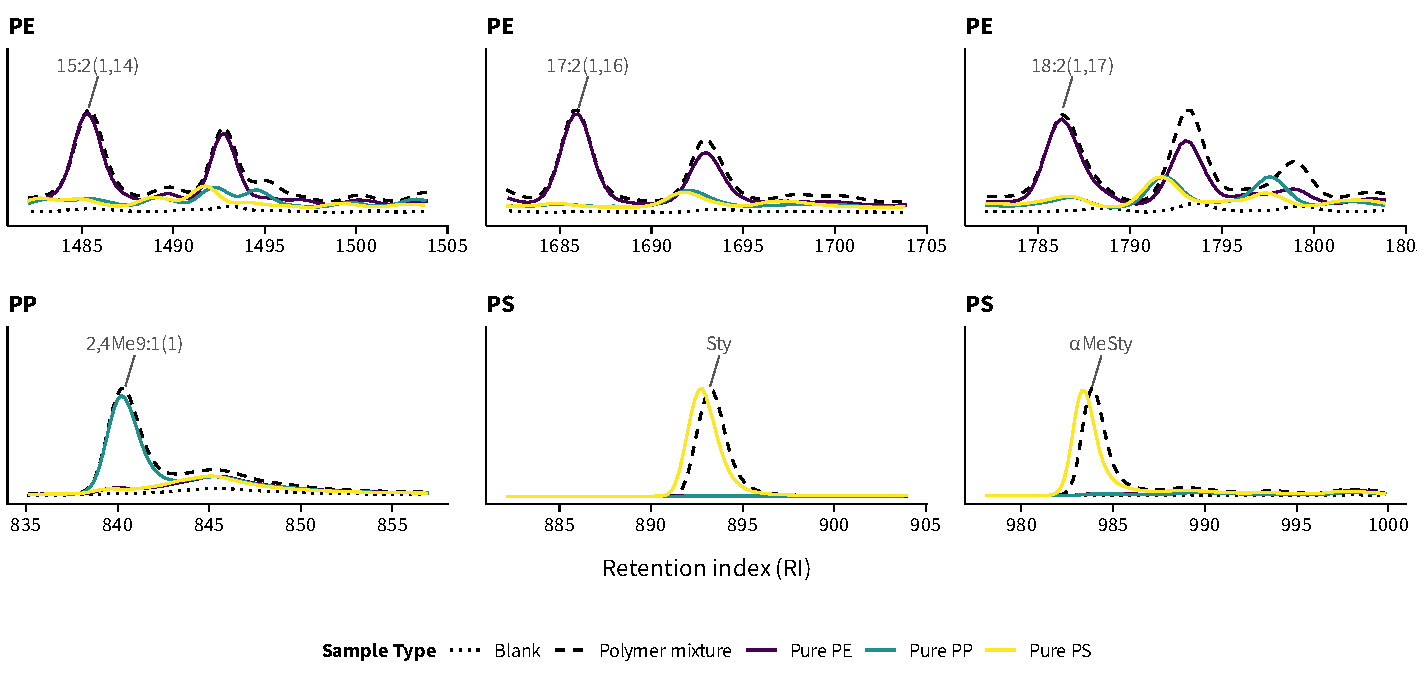
\includegraphics[width=\textwidth]{figures/py-selectivity1}
	\caption[Pyrogram sections of \ac{pe}, \ac{pp}, and \ac{ps} pyrolysates.]{Pyrogram sections of \ac{pe}, \ac{pp}, and \ac{ps} pyrolysates obtained by analyzing each individual polymer or a mixture of all three polymers (\SI{150}{\micro\gram\per\milli\liter}).}
	\label{fig:py-selectivity1}
\end{figure*}

\begin{figure*}[b]
	\centering
	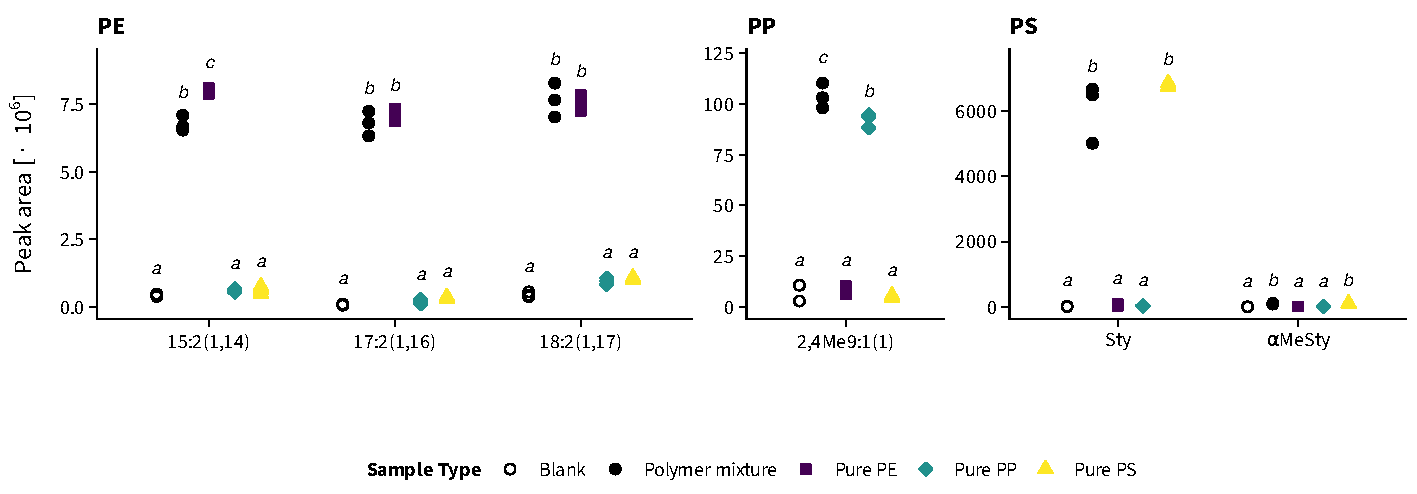
\includegraphics[width=\textwidth]{figures/py-selectivity2}
	\caption[Peak areas of \ac{pe}, \ac{pp}, and \ac{ps} pyrolysates.]{Peak areas of \ac{pe}, \ac{pp}, and \ac{ps} pyrolysates measured individually or in a mixture of all three polymers (\SI{150}{\micro\gram\per\milli\liter}); different letters (in italics) indicate significant differences between sample types for each pyrolysate ($p < 0.05$, Tukey).\\~}
	\label{fig:py-selectivity2}
\end{figure*}

To our knowledge, the possibility of polymers analyzed together and interfering with each other by formation of identical or chromatographically inseparable pyrolysates has so far only been described by \citet{FischerSimultaneous2017}. However, the authors neither tested potential interferences in their \ac{py-gc-ms} setup nor suggested a certain approach to counteract them. With our experimental design, we were able to show that \ac{pe}, \ac{pp}, and \ac{ps} can be selectively analyzed in a polymer mixture without interfering with each other by more than \SI{10}{\percent} at equal concentrations. Especially \ac{pp} quantified via 2,4Me9:1(1) may be slightly overestimated when \ac{pe} is present in large quantities. But since the \ac{pe} pyrolysate 17:2(1,16) was particularly robust against background signals from \ac{pp} or \ac{ps}, it would be possible to correct the overestimated \ac{pp} content for its \ac{pe} share.

\subsection{Matrix Interferences}\label{sec:matrix-interferences}

Extracting LUFA~2.2 and RefeSol 06-A with \ac{tcb}, but without adding plastic, resulted in background signals equivalent to \SIlist{70(10);31(4)}{\micro\gram\per\gram} \ac{pe}, respectively (Table~\ref{tab:py-matrix}). Interestingly, addition of the non-target plastics \ac{pet}, \ac{pvc}, \ac{pmma}, and \ac{twp} to LUFA~2.2 soil did not increase matrix interferences. With \SI{700(200)}{\micro\gram\per\gram}, the matrix-induced background signal in WR soil was about \numrange{10}{20} times higher than in LUFA~2.2. For soils with \iac{Corg} content exceeding \SI{2}{\percent}, namely RefeSol 06-A and WR, a prior cleanup step with methanol doubled \ac{pe} background levels. Similarly, Fenton digestion of WR soil resulted in matrix interferences equivalent to \SI{1000(200)}{\micro\gram\per\gram} \ac{pe}. Only flocculation with \ch{KAl(SO_4)_2} considerably reduced background levels to \SI{400(200)}{\micro\gram\per\gram}. Regardless of the extraction method and pretreatment, procedural blanks were below the estimated method \acp{lod} of \SI{5}{\micro\gram\per\gram}.
The \ac{pp} background extracted with \ac{tcb} was not detectable except for WR soil (\SI{100(100)}{\micro\gram\per\gram}). Similar to \ac{pe}, \ac{pp} levels doubled when applying a prior methanol cleanup step. However, \ch{KAl(SO_4)_2} flocculation and Fenton digestion were able to reduce matrix interferences below the \ac{lod}.
\Ac{ps} background levels in LUFA~2.2 soil were below the method \acp{lod} of \SI{3.2}{\micro\gram\per\gram}. In line with \ac{pe} and \ac{pp}, \ac{ps} contents slightly increased with the \ac{Corg} content of the soil. With respect to \acp{sd}, neither the methanol cleanup nor Fenton digestion changed the matrix-induced background considerably while \ch{KAl(SO4)2} decreased matrix interferences to non-detectable levels.

\begin{table*}
	\centering\footnotesize
	\caption[Matrix interferences of different soil types.]{Matrix interferences of different soil types (mean $\pm$ \ac{sd}).}\label{tab:py-matrix}
	\begin{tabular}{llS[table-format = 4(3)]S[table-format = 4(3)]S[table-format = 4(3)]S[table-format = 4(3)]}
		\toprule
		{Polymer} & {Soil} & \multicolumn{2}{l}{{Extraction procedure} [\si{\micro\gram\per\gram}]} \\
		\cmidrule(lr){3-6}
		& & {TCB only} & {Methanol cleanup} & {\ch{KAl(SO4)2} flocculation} & {Fenton digestion}\\
		\midrule
		PE & LUFA 2.2 & 70(10) &  &  &  \\
 & LUFA 2.2\textsuperscript{\textasteriskcentered} & 70(7) &  &  &  \\
 & RefeSol 06-A & 31(4) & 70(20) &  &  \\
 & WR & 700(200) & 1300(100) & 400(200) & 1000(200) \\
PP & LUFA 2.2 & 0(200) &  &  &  \\
 & LUFA 2.2\textsuperscript{\textasteriskcentered} & 0(100) &  &  &  \\
 & RefeSol 06-A & 0(0) & 32(100) &  &  \\
 & WR & 100(100) & 200(100) & 0(0) & 0(0) \\
PS & LUFA 2.2 & 2(4) &  &  &  \\
 & LUFA 2.2\textsuperscript{\textasteriskcentered} & 4(3) &  &  &  \\
 & RefeSol 06-A & 20(30) & 1(1) &  &  \\
 & WR & 7(3) & 12(4) & 0(4) & 8(3) \\

		\bottomrule
		\multicolumn{6}{p{.75\textwidth}}{\textsuperscript{*}with \SI{50}{\micro\gram\per\gram} non-target polymers (\SI{19}{\percent} \ac{pet}, \SI{11}{\percent} \ac{pmma}, \SI{41}{\percent} \ac{pvc}, and \SI{29}{\percent} \ac{twp}); indicator pyrolysates were 17:2(1,16) for \ac{pe}, 2,4Me9:1(1) for \ac{pp}, and $\alpha$MeSty for \ac{ps}.}
	\end{tabular}
\end{table*}

The matrix interferences identified in our study were generally comparable to those reported in previous thermoanalytical studies: \citet{DierkesQuantification2019} detected matrix interferences equivalent to \SIlist{140;210;50}{\micro\gram\per\gram} \ac{pe} in an artificial, inert matrix spiked with \SI{3}{\percent} of wood, leafs, or humic acids, respectively. The authors applied \ac{ase} with methanol and \ac{thf} prior to \ac{py-gc-ms} quantification via 15:2(1,14). Similarly, \citet{FischerSimultaneous2017} found their \ac{pe} and \ac{ps} pyrolyses affected by chitin, wood, wool, and cellulose, however, without quantifying potential interferences. For two natural soils with unreported \ac{Corg}, \SIrange{790}{850}{\micro\gram\per\gram} \ac{pe}, \SI{40}{\micro\gram\per\gram} \ac{pp}, and \SIrange{40}{50}{\micro\gram\per\gram} \ac{ps} were detected \citep{DierkesQuantification2019}. The question whether these levels came from matrix interferences or a contamination with plastic debris remained unresolved. By contrast, \citet{DumichenAnalysis2015} applied \ac{ted-gc-ms} and found that soil matrix with an unspecified \ac{Corg} did not induce any interferences. Since \citet{DumichenAnalysis2015,DumichenFast2017} determined \ac{pe} in a concentration range approximately three orders of magnitude higher than we did, contrasting findings are most likely attributed to the higher sensitivity of our \ac{py-gc-ms} setup. A comparison with existing microspectoscopic methods \citep{ScheurerMicroplastics2018,PiehlIdentification2018} remains difficult since results are typically reported as particle counts. Conversions from particle counts and sizes to mass concentrations are error-prone for the high uncertainties associated with the underlying assumptions on particle shapes and density distributions. That being said, background levels from \ac{ftir} analyses of Swiss floodplains were estimated at \SIrange{0}{55}{\micro\gram\per\gram} and averaged \SI{5}{\micro\gram\per\gram}, which is \numrange{1.2}{15} times lower than the matrix interferences identified in our study.

Besides a facilitated sample handling, dissolution of \ac{pe}, \ac{pp}, and \ac{ps} in \ac{tcb} offers the advantage of restricting the amount of other polymers and interfering matrix being dissolved along with the analytes and transferred into the \ac{py-gc-ms} system. Apart from our three target polymers, \ac{tcb} is recommended as \ac{sec} solvent only for poly(ethylene-vinyl acetate), polythiophene, and other polyolefins \citep{BivensPolymertoSolvent2016}. In addition, only compounds thermally decomposing between \SIrange[range-phrase = { and }]{300}{750}{\degreeCelsius} were passed to our \ac{gc-ms}, which may have further reduced the potential for interferences.

In spite of that, we found particularly high matrix interferences for \ac{pe} in WR soil, a pristine forest soil with \SI{5.16}{\percent} \ac{Corg}. The two agricultural soils with \SI{<2.5}{\percent} \ac{Corg} showed considerably lower background signals.
This is not surprising since up to \SI{9}{\percent} of soil \ac{Corg} consists of \ch{(CH2)_{$n$}} chains of \numrange{25}{30} units \citep{HuPoly2000} as, for example, present in suberins, cutins, or microbial cell membranes. Based on the \ac{Corg} of our reference soils, this fraction could potentially induce interferences equivalent to \SIrange{1500}{4500}{\micro\gram\per\gram} \ac{pe}. Just by using \ac{tcb} as an extraction agent, we were able to reduce potential interferences by a factor of \numrange{5}{20}. In comparison with that, prior Fenton digestion or methanol cleanup rather mobilized than removed interfering matrix constituents, for instance by cell lysis, which was indicated by elevated \ac{pe} background levels from both pretreatments. The differences between both pretreatments may be attributed to the oxidization potential of Fenton reagent that most likely made available but at the same time removed a larger fraction of interfering matrix constituents than methanol.
Here, existing \ac{ase} applications with three rinsing cycles of \SI{15}{\milli\liter} methanol per \SI{1}{\gram} of sample at \SI{100}{\degreeCelsius} \citep{FullerProcedure2016,DierkesQuantification2019} may be superior to our simplified batch setup. But matrix interferences from such extraction setups have not been quantified for organic rich soils yet.
Besides that, it cannot be excluded that reference soils may have been contaminated with plastic debris on-site or during packaging and shipping, thereby, mistaking a potential plastic contamination for matrix interferences. This could only be assessed by characterizing soil organic matter fractions from soil databases dating back to times before the introduction of today's consumer plastics. Based on these findings, further efforts should be made to reduce interferences from specific soil constituents, for instance by using an advanced flotation and filtration apparatus, molecular sieves, dispersive \ac{spe}, or on-line transesterification and evaporation of lipid-like substances with \ch{BF3} or \ac{tmsh} prior pyrolysis. Moreover, further research will need to test alternative solvent mixtures to extend the applicability of our \ac{py-gc-ms} approach to a wider range of polymer types.

\subsection{Plastic Recovery from Soil}

As outlined above, matrix interferences equivalent to \SI{>400}{\micro\gram\per\gram} \ac{pe} exceeded the spiked polymer content by a factor of \numrange{2}{4}. In those cases, the calculation of matrix-corrected recoveries was not meaningful and data were thus excluded from further examination (Figure~\ref{fig:py-recovery}).
\Ac{pe} recovered from LUFA~2.2 with \ac{tcb} only ranged from \SIrange[range-phrase = { to }]{80}{110}{\percent}. The recoveries were independent of the spiking level, and the addition of non-target polymers did not influence the recovery of \ac{pe}. For RefeSol 06-A, recoveries with \ac{tcb} were slightly lower than in LUFA~2.2 (\SIlist{61;70}{\percent}). The methanol cleanup decreased the recovery to \SIlist{26;55}{\percent}. Due to the high matrix interferences discussed in Section~\ref{sec:matrix-interferences}, \ac{pe} recoveries from WR soil could only be evaluated for samples flocculated with \ch{KAl(SO4)2} prior to \ac{tcb} extraction, and the recovery was very low (\SI{10(10)}{\percent}).
Extracting \ac{pp} from LUFA~2.2 and RefeSol 06-A soil using \ac{tcb} yielded recoveries of \SIrange{100}{160}{\percent}. At \SI{50}{\micro\gram\per\gram} spiking level, recoveries were higher and varied more than at \SI{250}{\micro\gram\per\gram}. In line with \ac{pe}, the methanol pretreatment decreased recoveries to \SIlist{63;80}{\percent}. In WR soil, only \SI{30(20)}{\percent} of \ac{pp} were recovered after \ch{KAl(SO4)2} flocculation. Prior Fenton digestion increased recoveries to \SIlist{110;140}{\percent}.
\Ac{ps} recoveries ranged from \SIrange[range-phrase = { to }]{77}{119}{\percent}, except for the Fenton digestion of WR soil (\SI{130(10)}{\percent}) and \ac{tcb} extraction of RefeSol 06-A at the lower spiking level of \SI{50}{\micro\gram\per\gram} (\SI{46(7)}{\percent}).

\begin{figure*}[t]
	\centering
	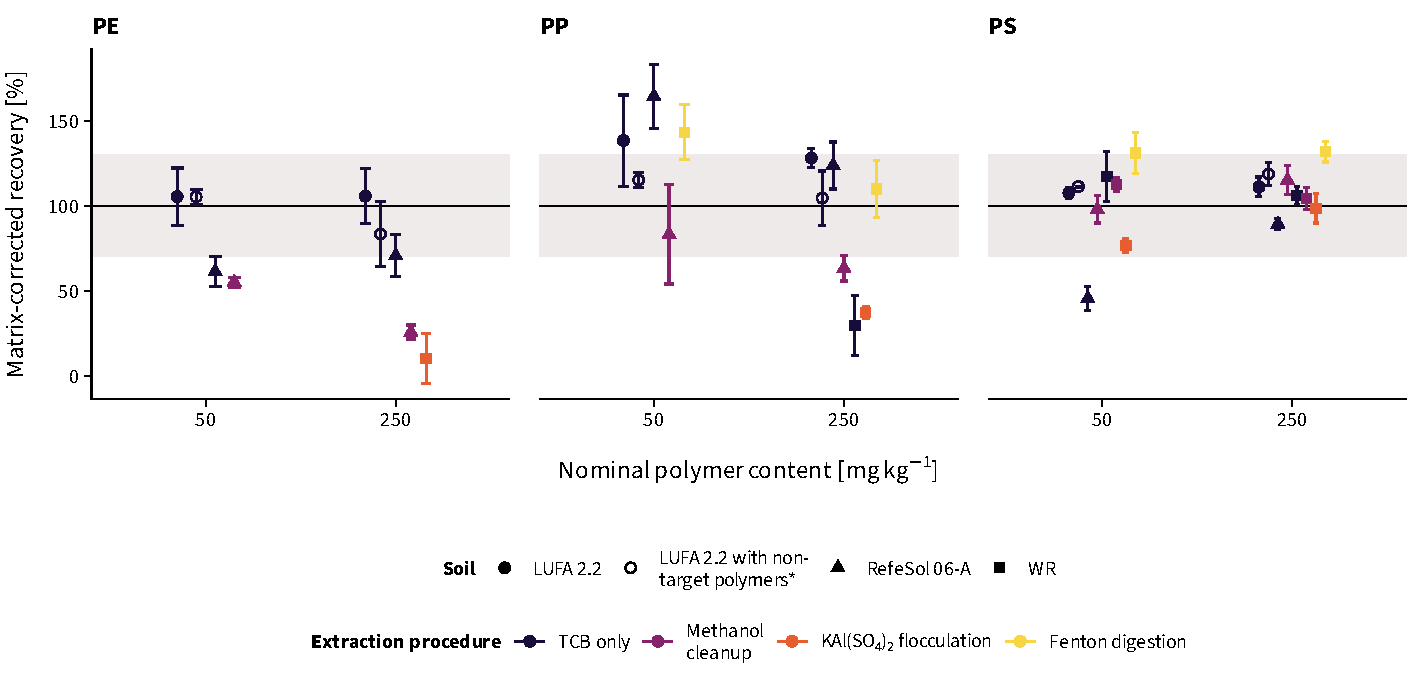
\includegraphics[width=\textwidth]{figures/py-recovery}
	\caption[Recoveries of \ac{pe}, \ac{pp}, and \ac{ps} from different soil types corrected for matrix interferences.]{Recoveries of \ac{pe}, \ac{pp}, and \ac{ps} from different soil types (mean $\pm$ \ac{sd}) corrected for matrix interferences (Table~\protect\ref{tab:py-matrix}); the gray band marks the \SIrange{70}{130}{\percent} range acceptable for recovery experiments; \textsuperscript{\textasteriskcentered}\SI{50}{\micro\gram\per\gram} consisting of \SI{19}{\percent} \ac{pet}, \SI{11}{\percent} \ac{pmma}, \SI{41}{\percent} \ac{pvc}, and \SI{29}{\percent} \ac{twp}.}
	\label{fig:py-recovery}
\end{figure*}

In summary, \ac{tcb} extractions without any pretreatment performed best (\SIrange{70}{128}{\percent} recovery), particularly at \SI{250}{\micro\gram\per\gram} spiking level from soils with less than \SI{2.5}{\percent} \ac{Corg}. \Ac{pp} contents were slightly overestimated due to the aforementioned interference with \ac{pe} (Section~\ref{sec:selectivity}). Although \ch{KAl(SO4)2} effectively immobilized interfering matrix constituents, it concomitantly reduced \ac{pe} and \ac{pp} recoveries. This was potentially due to matrix floccules entrapping plastic debris, hence making it inaccessible to \ac{tcb} extraction. Similarly, low recoveries resulting from the methanol cleanup were most likely attributed to the discarding of supernatant methanol after rinsing, which probably also removed some plastic debris from the soil. Interestingly, prior Fenton digestion led to elevated recoveries, which contrasts \citet{HurleyValidation2018} who found Fenton reagent performing best in terms of organic matter removal and preservation of plastic particles prior to \ac{ftir} imaging. However, our findings are in line with previous thermoanalytical studies that obtained recoveries of \SIrange{80}{130}{\percent} when extracting \ac{pe}, \ac{pp}, and \ac{ps} with dichloromethane and \ac{thf} from solid matrices after an initial methanol cleanup \citep{FullerProcedure2016,DierkesQuantification2019}. In contrast to our study, \citet{FullerProcedure2016} used about \numrange{20}{100} times higher spiking levels (\SI{5}{\milli\gram\per\gram}) and \citet{DierkesQuantification2019} extracted \SIlist{50;750}{\micro\gram\per\gram} microplastics from an artificial sample containing \SI{3}{\percent} humic acids in sea sand. In such an artificial matrix, interferences are less likely to occur than in natural soil with its large variety of substance classes like natural polymers, lipids, or proteins.

\section{Conclusions}

Dissolving the three most environmentally relevant polymers \ac{pe}, \ac{pp}, and \ac{ps} in \ac{tcb} for the direct quantification of liquid sample aliquots via \ac{py-gc-ms} facilitated the preparation of calibration curves, simplified and sped up sample handling, reduced the risk of contamination, and allowed for the selective extraction of plastic debris from several grams of solid matrix.
The latter enabled us to account for the heterogeneity of soil while minimizing interferences from non-target polymers and soil matrix. Yet, one organic-rich forest soil inflated matrix interferences so that the method currently remains limited to agricultural soil with less than \SI{2.5}{\percent} \ac{Corg}. Further method development is necessary to reduce such matrix interferences in order to comply, for example, with 2002/657/EC criteria for residual analysis by the \citet{EuropeanCommissionCommission2002}. Follow-up studies will also need to assess to what extent the solubility of plastic debris in \ac{tcb} may be affected by the degree of polymer crosslinking, varying molar weights, or changes in particle crystallinity and surface properties that are likely to occur during plastic aging in soil.

Once this is resolved, our new \ac{py-gc-ms} method may be applied for routine analyses and screening studies to better understand the occurrence and fate of plastic debris in agricultural systems, for instance, to scrutinize whether agricultural plastic films function as source for plastic debris in soil. After an initial screening, selected hot spots or points of interest could be analyzed by complementary \ac{ftir} or Raman microspectroscopy for additional information about particle shapes and sizes.
